% \documentclass[bachelor,nocolorlinks, printoneside]{seuthesis} % 本科
\documentclass[master]{seuthesis} % 硕士
% \documentclass[doctor]{seuthesis} % 博士
% \documentclass[engineering]{seuthesis} % 工程硕士
\usepackage{CJK,CJKnumb}
\usepackage{amsmath}
\usepackage{amsfonts} 
\usepackage{bm} 
\usepackage{algorithm}
\usepackage{algorithmicx}
\usepackage{algpseudocode}
\usepackage{subfigure}

\floatname{algorithm}{算法}
\renewcommand{\algorithmicrequire}{\textbf{输入:}}
\renewcommand{\algorithmicensure}{\textbf{输出:}}
 % 这里是导言区

\begin{document}
\categorynumber{000} % 分类采用《中国图书资料分类法》
\UDC{000}            %《国际十进分类法UDC》的类号
\secretlevel{公开}    %学位论文密级分为"公开"、"内部"、"秘密"和"机密"四种
\studentid{09013000}   %学号要完整,前面的零不能省略。

\title{一种TDD/FDD下低时延宽带无线信道密钥生成系统研究}{}{Deep learning in greek alphabet}{subtitle}
\author{袁瑞}{Rui Yuan}
% \advisor{彭林宁}{副研究员}{Linning Peng}{Associate Prof.}  % 没有
\coadvisor{彭林宁}{副教授}{Linning Peng}{Associate Prof.}

% \degree{工学硕士} % 详细学位名称
\major[12em]{网络空间安全}
\defenddate{答辩日期}
\authorizedate{学位授予日期}
\department{网络空间安全}{department name}
\duration{2017年9月—2020年6月}
\address{东南大学}
% \thanks{本论文获国家XXX计划项目(2012AA00A00)和国家杰出青年科学基金项目(01234567)资助。}
\maketitle

\begin{abstract}{希腊字母,腓尼基字母,语言,深度学习}
希腊字母源自腓尼基字母。腓尼基字母只有辅音,从右向左写。希腊语的元音发达,希腊人增添了元音字母。因为希腊人的书写工具是蜡板,有时前一行从右向左写完后顺势就从左向右写,变成所谓“耕地”式书写,后来逐渐演变成全部从左向右写。字母的方向也颠倒了。罗马人引进希腊字母,略微改变变为拉丁字母,在世界广为流行。希腊字母广泛应用到学术领域,如数学等。

希腊字母是希腊语所使用的字母,是世界上最早的有元音的字母,也广泛使用于数学、物理、生物、天文等学科。俄语等使用的西里尔字母也是由希腊字母演变而成。希腊字母进入了许多语言的词汇中,英语单字“alphabet”(字母表),源自拉丁语“alphabetum”,源自希腊语“αλφαβητον”,即为前两个希腊字母α(“Alpha”)及β(“Beta”)所合成,三角洲(“Delta”)这个词就来自希腊字母Δ,因为Δ是三角形。
\end{abstract}

\begin{englishabstract}{Greek Alphabet, Phoenician Alphabet, Language, Deep Learning}
The Greek alphabet has been used to write the Greek language since the late 9th century BC or early 8th century BC It was derived from the earlier Phoenician alphabet, and was the first alphabetic script to have distinct letters for vowels as well as consonants. It is the ancestor of the Latin and Cyrillic scripts.Apart from its use in writing the Greek language, in both its ancient and its modern forms, the Greek alphabet today also serves as a source of technical symbols and labels in many domains of mathematics, science and other fields.

In its classical and modern forms, the alphabet has 24 letters, ordered from alpha to omega. Like Latin and Cyrillic, Greek originally had only a single form of each letter; it developed the letter case distinction between upper-case and lower-case forms in parallel with Latin during the modern era.
\end{englishabstract}

\tableofcontents

% \begin{terminology}
% \begin{table}[h]
% \renewcommand\arraystretch{1.5}
% %\Large
% \begin{tabular}{>{\LARGE}m{0.2\textwidth} <{\centering}m{0.7\textwidth}}
% a & 如同汉字起源于象形,拉丁字母表中的每个字母一开始都是描摹某种动物或物体形状的图画\\

% b&和A一样,字母B也可以追溯到古代腓尼基。在腓尼基字母表中B叫beth,代表房屋,在希伯来语中B也叫beth,也含房屋之意。\\

% c& 字母C在腓尼基人的文字中叫gimel,代表骆驼。它在字母表中的排列顺序和希腊字母Γ(gamma)相同,实际上其字形是从后者演变而来的。C在罗马数字中表示100。\\

% d&D在古时是描摹拱门或门的形状而成的象形符号,在古代腓尼基语和希伯来语中叫做daleth,是“门”的意思,相当于希腊字母Δ(delta)。\\

% \end{tabular}
% %\caption{my table}
% \end{table}
% \end{terminology}

\begin{Main} % 开始正文

\chapter{绪论}
\section{研究背景和意义}

无线通信在民事和军事应用中已经发挥着不可替代的作用,研究无线通信的安全性具有重要研究价值。无线网络由于接入层的开放性,因此容易遭受攻击。无线网络的安全性通常由传统密码学保证,比如公钥基础设施(PKI)。PKI被广泛应用于保护计算机网络,但并不适用于物联网设备。首先,PKI是依赖高时间复杂度算法,而物联网设备通常是低功耗设备。此外,PKI的基石来自数论,比如大整数分解问题,随着量子计算的发展,此类问题或被攻破。

\subsection{当前无线通信网络中存在的问题}

由于无线媒介的共享特性,无线通信中的信息传输可能遭到窃听、篡改和伪造。为了保护信息的完整、可信,在无线网络中需要建立会话密钥。

但是无线通信网络的开放性、脆弱性和拓扑性,使得无线通信网络极易遭受攻击:

1. 相对于有线网络,由于物理边界的缺失,无线通信网络的广播特性使得范围内任意用户可以接入网络,使得传输信息容易被非法用户窃听,并且难以察觉窃听者的地点。
2. 无线信号的叠加特性,使得非法用户有能力释放干扰信号或者伪造信号给合法用户,降低通信得到可靠性,破坏用户接收数据的完整性
3. 无线通信网络拓扑具有灵活性和移动性,传统的密钥分发方案并不适用于动态变化的网络拓扑结构,在资源受限的节点网络中,影响更为突出。

另外,传统的安全机制主要通过协议上层(应用层、传输层)的加密来实现,传统安全通信需要第三方机构注册证书、分发密钥,然后通过会话密钥进行会话。传统安全通信是“有条件”的安全,因为其安全性是建立在非法用户的计算能力有限的基础上,随着算力提高和硬件发展,密码学相关算法或被攻破。传统安全通信即使保证上层协议的安全,也无法完全避免物理层的恶意干扰,因此物理层安全的相关研究应运而生,出现了大量物理层的安全机制相关的研究。

物理层安全机制可以从根本上解决无线通信的安全性问题,与传统安全机制相比,物理层安全从物理层实现信息的安全处理。在物理层安全机制的研究工作中,基于密钥的物理层安全机制将传统安全机制和物理层安全机制相结合的方案,具有高可行性和高可靠性的特点,其特点是通过无线信道的特性进行密钥生成的相关工作,最后提供密钥给上层应用直接使用。

\subsection{无线信道密钥生成技术}

无线信道密钥生成技术属于物理层安全的范畴,通过利用合法通信双方之间的信道特性,估计无线信道特征,量化生成会话密钥,进而将会话密钥提供给上层协议使用。

物理层安全不同于传统密码学,目前演化成了两个分支,无密钥安全和基于密钥的安全机制。其中无密钥实现复杂,需要苛刻的信道条件。基于密钥的安全机制是将物理层安全和传统安全机制结合的安全方案。在无线通信网络中,无线信道通信的特性有以下特性:

\begin{itemize}
    \item \textbf{短时互易性}。在时分双工(Time Division Duplex, TDD)系统中,通信双方的上下行信道在相干时间内具有相似的信道特征。
    \item \textbf{随机性}。随着时间变化,周围环境中物体的移动会扰动信道,造成信道随机变化,通过信道特征提取的密钥自然也具有随机性,因此每次协商的密钥都将不可预测,这符合安全机制对密钥的要求。
\end{itemize}

由于无线通信信道具有上述特性,因此在物理层协商生成安全、可靠的密钥是可行的,一方面不依赖第三方传输机构,另一方面计算复杂度较小。

\section{国内外研究现状}

无线通信的广播特性允许范围内其他用户接收信号,因此容易遭受攻击。攻击者可以利用该特性进行被动攻击,比如窃听和监控信息、分析网路流量,或者进行主动攻击,比如修改消息、伪造认证、重放攻以及拒绝服务(Dos)攻击\cite{Zhang2016Key}。传统的安全工作依赖于公钥算法体系,比如RSA等算法,因为窃听者破译信息所需时长远远超过信息本身的价值,由此保障后向安全。

图\ref{wirelss-network-security}所示传统加密方法包含对称加密和非对称个加密,对称加密算法使用相同的一对密钥,可以用于对加密时间要求较高的场景;非对称加密算法使用一对公钥和私钥,通常用于密钥分发。

传统加密算法有以下几个问题。首先,传统加密算法依赖一些数学问题的计算难度,比如离散对数问题。随着硬件发展和算力的大幅提升,通过计算难度保证安全不再可取。此外,传统加密算法需要一个可信的密钥管理设施,并不适用于去中心化的无线传感器网络(WSN)和无线自组网络,并且传感器节点的计算能力有限。

即使通信协议的上层应用了传统加密算法,物理层也应当加强无线安全、抵抗攻击。物理层安全(PLS)利用无线信道的不可预测性和随机性来达到信息论安全。如图\ref{wirelss-network-security}所示,PLS方法包括无密钥安全和基于密钥的安全机制。在Wyner提出的窃听信道模型中,无密钥安全不需要加密密钥,而是通过合法用户和窃听者之间不同的信道特性来保证安全\cite{6739367}。合法用户需要窃听用户的瞬态或者稳态信道状态信息(CSI),但是在生产环境中,获取窃听用户的瞬态和稳态信号十分复杂。

基于密钥的安全机制追随到1919年提出的Vernam加密,即一次一密\cite{vernam1922secret}。之后,香农为完全保密提出理论基础\cite{shannon1949communication}。当密钥Key的信息大于等于消息M的信息时,消息M可以被编码成码字C,并不会泄露任何消息,即

\begin{equation}
    H(M|C) = H(M)
\end{equation}

其中,$H(\cdot)$表示熵。然而,在生产环境中,在合法用户之间协商不可重用的随机密钥是非常困难的。一种可行的方案是,将密钥生成和对称加密结合在一起形成混合加密系统。

\begin{figure}[htbp!]
    \centering 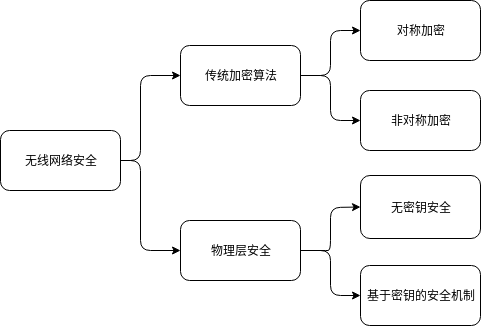
\includegraphics[width=0.9\textwidth]{images/wireless-network-security} 
    \caption{无线网络安全}
    \label{wirelss-network-security}
\end{figure}

本文研究无线信道密钥生成,即利用无线信道的随机性来生成密钥。和公钥体系利用数论问题保证安全性不同,无线密钥生成的安全性基于信息论。因为它基于无线信道的随机性\cite{ahlswede1993common}\cite{maurer1993secret},并且不需要借助其他用户的信息。以上所提及方法的优缺点列在表\ref{comparison-different-schemes}。

\begin{table}[]
    \begin{tabular}{|l|l|l|l|l|}
    \hline
    方法 & 描述 & 实现复杂度 & 优点 & 缺点 \\ \hline
    对称加密 & 合法通信双方用对称密钥加密数据 & 易实现 & 算法复杂度低 & 提前协商会话密钥;计算安全性 \\ \hline
    非对称加密 & 合法通信双方使用一对公私钥协商会话密钥 & 易实现 & 可用于协商会话密钥 & 计算安全性;依赖PKI;不适于低功耗设备 \\ \hline
    无密钥安全 & 合法通信双方通过设计编码和信道特性避免泄露信息 & 实现复杂 & 信息论安全;无需密钥的安全传输 & 依赖窃听者的CSI \\ \hline
    基于密钥的安全机制 & 合法通信双方利用信道的随机性生成密钥 & 易实现 & 信息论安全;轻量;无需第三方参与 & 受限于信道特性本身 \\ \hline
    \end{tabular}
    \caption{不同方法的比较
    \label{comparison-different-schemes}}
\end{table}

1993年Maurer等人理论上提出密钥生成\cite{ahlswede1993common}\cite{maurer1993secret}。密钥生成的模型如图\ref{}所示。图\ref{}中Alice和Bob需要建立一个安全的加密通道,窃听者Eve与Alice相距d厘米,并监听了所有传输过程。Alice、Bob和Eve可以分别接收到信号$X^n = (X_1, ..., X_n)$,$Y^n = (Y_1, ..., Y_n), Z^n = (Z1, ..., Z_n)$。Alice和Bob在公共信道上交换消息s,Eve同样可以接收到消息s。对任何$\epsilon > 0$和足够大的$n$,如果存在$K^A = g_A(X^n, s)$和$K^B = g_B(Y^n, s)$使得密钥生成体系满足

\begin{eqnarray}
    Pr(K^A \neq K^B) < \epsilon \label{keyrate1} \\
    \frac{1}{n}I(K^A; s, Z^n) < \epsilon \label{keyrate2} \\
    \frac{1}{n}H(K^A) > R - \epsilon \label{keyrate3} \\
    \frac{1}{n}log[\mathcal{K}] < \frac{1}{n}H(K^A) + \epsilon \label{keyrate4}
\end{eqnarray}

那么式中R即可达密钥速率,其中$I(\cdot)$表示互信息,$\mathcal{K}$表示密钥key的字母表。公式\ref{keyrate1}表示Alice和Bob生成相同密钥的可能性;公式\ref{keyrate2}表示通过公共信道传输消息,不会泄露给窃听者Eve,从而保证密钥安全性;公式\ref{keyrate4}确保密钥是均匀分布。最大可达密钥速率可以用密钥容量定义,

\begin{equation}
    C_K = min[I(X;Y), I(X, Y|Z)]
\end{equation}

目前已经有一些研究工作实现上述理论。1995年第一个实际的密钥生成协议被提出\cite{hershey1995unconventional},之后陆续出现大量研究无线密钥生成的相关工作。\citet{WangSurvey}的第四章从信息论角度阐述了无线密钥生成。\citet{WangSurvey}将信道探测和量化合并为一个步骤来研究。\citet{zeng2015physical}介绍了密钥生成技术存在的机遇和挑战,但是未涉及到具体实现细节。尽管\citet{ren2011secret}总结了一些密钥生成方法,比如基于接收信号强度(RSS)和基于信道相位的方法,但是由于之后密钥生成方法和技术迅速发展,所以仍然需要对密钥生成方法进行梳理。本文会对密钥生成技术做一个完整的文献综述。同时,本文会对密钥生成技术的未来发展提出相关建议。

\section{研究内容和方法}

无线信道密钥生成协议通常包含四个步骤,信道探测、特征量化、信息调和以及隐私放大:

\begin{itemize}
    \item \textbf{信道探测}。信道探测是测量无线信道并提取无线信道特征的过程。通信双方互相收发导频信号,并从接收到的导频信号中提取信道特征。
    \item \textbf{特征量化}。特征量化是将无线信道特征通过预处理、归一化、量化等操作得到比特流的过程。由于提取的无线信道特征受到接收端增益等参数的影响,所以需要预处理、归一化等操作来使得双方探测的信道特征更加相近。之后,再量化成比特流。
    \item \textbf{信息调和}。信息调和是利用无线信道特征作为随机密钥源并结合合理可靠的交互协议生成会话密钥的过程。通信双方在探测信道之后,量化信道得到密钥,通过公共信道的交互协议去除密钥中的不一致比特,得到完全一致的会话密钥。
    \item \textbf{隐私放大}。隐私放大是进一步提高密钥随机性和可靠性、去除密钥中信道相关信息的过程。通过单向哈希函数等方法,可以移除密钥中隐藏的信道信息,进一步提高密钥的安全性。
\end{itemize}

本文基于GNURadio软件无线电开发平台,实现一种TDD/FDD下低时延宽带无线信道密钥生成系统。本文系统信道探测部分分为两种模式,一种TDD模式,另一种FDD模式,并研究两种模式下的信道互易性、密钥安全性等,设计TDD模式和FDD模式下低时延的会话密钥协商技术。无论是TDD还是FDD,其核心都是通信双方在相干时间内获取对端发射的导频信号,并从接收的导频信号中分析和提取信道特征。两种模式除了信道探测部分不同,其余三部分均比较相似。

TDD模式和FDD模式的主要不同点是收发导频信号的机制不同。TDD模式下,通信双方工作在同一频率,相干时间内,两个发送端发射的电磁波经管相同的信道衰落;FDD模型下通信双方工作在不同频率,收发导频信号几乎发生在同时。由于合法通信双方的通信信道在空间上唯一性,所以即便第三方窃听者监听到任意一方发送的导频信号,也无法分析出通信双方之间的CSI信息,以此保障密钥的安全。

无论是TDD模式还是FDD模式,通信双方提取出CSI之后的主要过程是相似的:量化、调和。由于无线信道的短时互易性,通信双方的CSI是相近的,在量化之后得到的比特流也是相似的,但是由于信道在探测时隙内发生变化以及周围环境中的干扰等各种因素,双方提取的密钥又是不完全一致的。因此需要进一步调和,去除不一致比特或者纠正错误比特。调和之后,通信双方会获取一致的比特流,为了进一步去除比特流中的信道信息,进行隐私放大得到最终的会话密钥。

GNURadio是软件无线电开发平台,被广泛应用于音频处理、移动通信、卫星追踪、GSM网络等计算机软件\cite{Blossom2004GNU},用户可以在GNURadio平台上设计、仿真以及部署高性能无线电的软件无线电系统。本文基于GNURadio软件无线电开发平台和USRP N210硬件,设计TDD/FDD下低时延宽带无线信道密钥生成系统,并验证生产环境下无线密钥生成技术的可靠性和安全性。

在现有关于无线密钥生成技术的研究中,无线密钥生成技术的理论和仿真居多,在实际生产环境中实现并验证的研究并不多见。本文基于GNURadio软件无线电平台,设计和开发了TDD/FDD模式下低延迟无线密钥生成系统,并在不同场景下采集数据,通过分析CSI的相关性、信道随机性、密钥随机性、信息泄露等五种指标,充分验证无线密钥生成技术在实际环境中使用的安全性和可靠性。

\section{本文主要内容与章节安排}

本文主要研究无线信道密钥生成技术及其实际应用。文章先介绍了无线信道密钥生成技术的研究背景,并概述国内外无线信道密钥生成技术的研究现状,在现有研究基础上,基于GNURadio软件无线电平台,设计和开发TDD/FDD模式下低延迟无线密钥生成系统,系统达到todo的密钥生成速率,平均每次密钥协商过程todo秒,并提出相应的系统性能评估指标,在多种场景下评估系统性能并分析系统优缺点。

\subsection{本文主要内容}

本文完成的主要工作包括:

(1)分析无线密钥生成技术的意义和背景,介绍无线密钥生成技术的国内外研究现状以及相关问题
(2)基于无线密钥生成技术的理论,设计完整的无线密钥生成技术方案,搭建TDD/FDD无线密钥生成系统。
(3)基于TDD/FDD无线密钥生成系统,研究不同场景下无线密钥生成系统的安全性和可靠性,通过多次实验分析通信参与者CSI的相关性、无线信道随机性、密钥的随机程度、信息泄露量,支撑无线密钥生成技术的实际应用意义。
(4)todo 射频指纹?
(5)todo 通过某些技术提高互易性?

\subsection{本文章节安排}

根据以上研究内容,本文分为todo章,具体章节安排如下:

todo

\chapter{无线密钥生成系统的理论基础}

本章节主要介绍无线密钥生成系统的理论基础。无线密钥生成系统的本质是利用无线信道的短时互易性、时空唯一性进行密钥生成的工作,在信道探测之后,量化生成的CSI,并进一步调和和隐私放大。另外本章介绍了系统生成密钥的评估标准,通过CSI相关性、信道随机性、密钥随机性和信息泄漏率等五个方面评估系统生成密钥的可靠性和安全性。

\section{无线信道特性}

\subsection{无线信道的短时互易性}

在TDD系统的上下行链路中,假设通信双方Alice和Bob以及窃听者Eve。在相干时间内,Alice和Bob互相发射的信号经过相同的信道衰落,因此由此估计出的信道具有互易性。

在图\ref{wireless-channel}中,Alice和Bob之间上下行链路的频率响应分别为$H_{ab}(t)$和$H_{ba}(t)$,相干时间内有$H_{ab}(t) = H_{ba}(t)$。假设在一次信道探测过程中,探测时隙为$\Delta t$,相干时间$\tau$内,Alice和Bob分别测量信道为$\tilde{H_{ba}(t)}$和$\tilde{H_{ab}(t)}$,当$ \Delta t < \tau $时有,

\begin{equation}
    H_{ba}(t) \approx H_{ab}(t + \Delta t)
\end{equation}

即双方探测的信道是近似相同的,因此通信双方可以通过利用无线信道的短时互易性来探测信道,进而结合其他协议生成相同的一致密钥。

同时,由于射频端的非线性特性、信道估计引入的误差、信道的时变性等因素\cite{guillaud2005practical},通信双方对信道的探测结果会有波动性差异:

\begin{itemize}
    \item 器件非线性。射频器件的非线性会导致I/Q路不平衡,如图\ref{iq_imbalance}所示,IQ不平衡会直接影响信号的发射和接收。在TDD系统中,收发两端的IQ不平衡会给上下行信道估计的互易性带来损失。
    \item 信道时变性。在相干时间内,无线信道具有短时互易性。但是由于无线信道的时变性,当双方探测信道的时隙超过信道相干时间,上下行信道估计结果会出现一定差异。
    \item 信道估计引入的误差。在基于导频的信号估计中,通过接收的导频信号和发射的导频信号做数学运算估计信道的频率响应,算法原理是通过最小化均方误差来估计信道,因此算法本身具有一定误差。
    \item 其他。另外,还有上下行链路的加性噪声也会对接收的信号有加性影响,不同频率子载波也会导致上行链路的差异等等。
\end{itemize}

\begin{figure}[htbp!]
    \centering 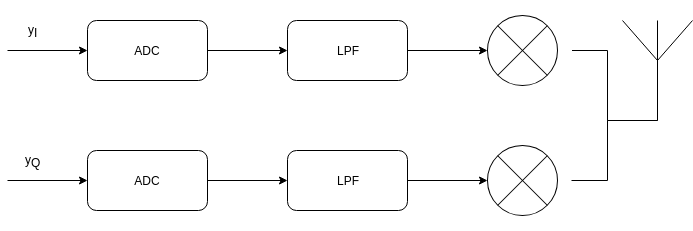
\includegraphics[width=0.9\textwidth]{images/iq_imbalance} 
    \caption{发射机存在的IO不平衡}
    \label{iq_imbalance}
\end{figure}


目前已经有相关工作研究如何对信道互易性的损失进行补偿,比如信道预测技术对信道互易性进行补偿,其原理是利用信道探测数据本身对未来时间的信道数据做出预测\cite{heidari2010adaptive}。另外基于信道互易性的MIMO预处理技术也可以一定程度上提高信道互易性,进而提高密钥一致性。针对IQ不平衡致使的信道互易性损失,可以估计系统中的不平衡参数,使相邻子载波的均方误差最小\cite{tubbax2005compensation}。

\subsection{无线信道的时空唯一性}

\begin{figure}[htbp!]
    \centering 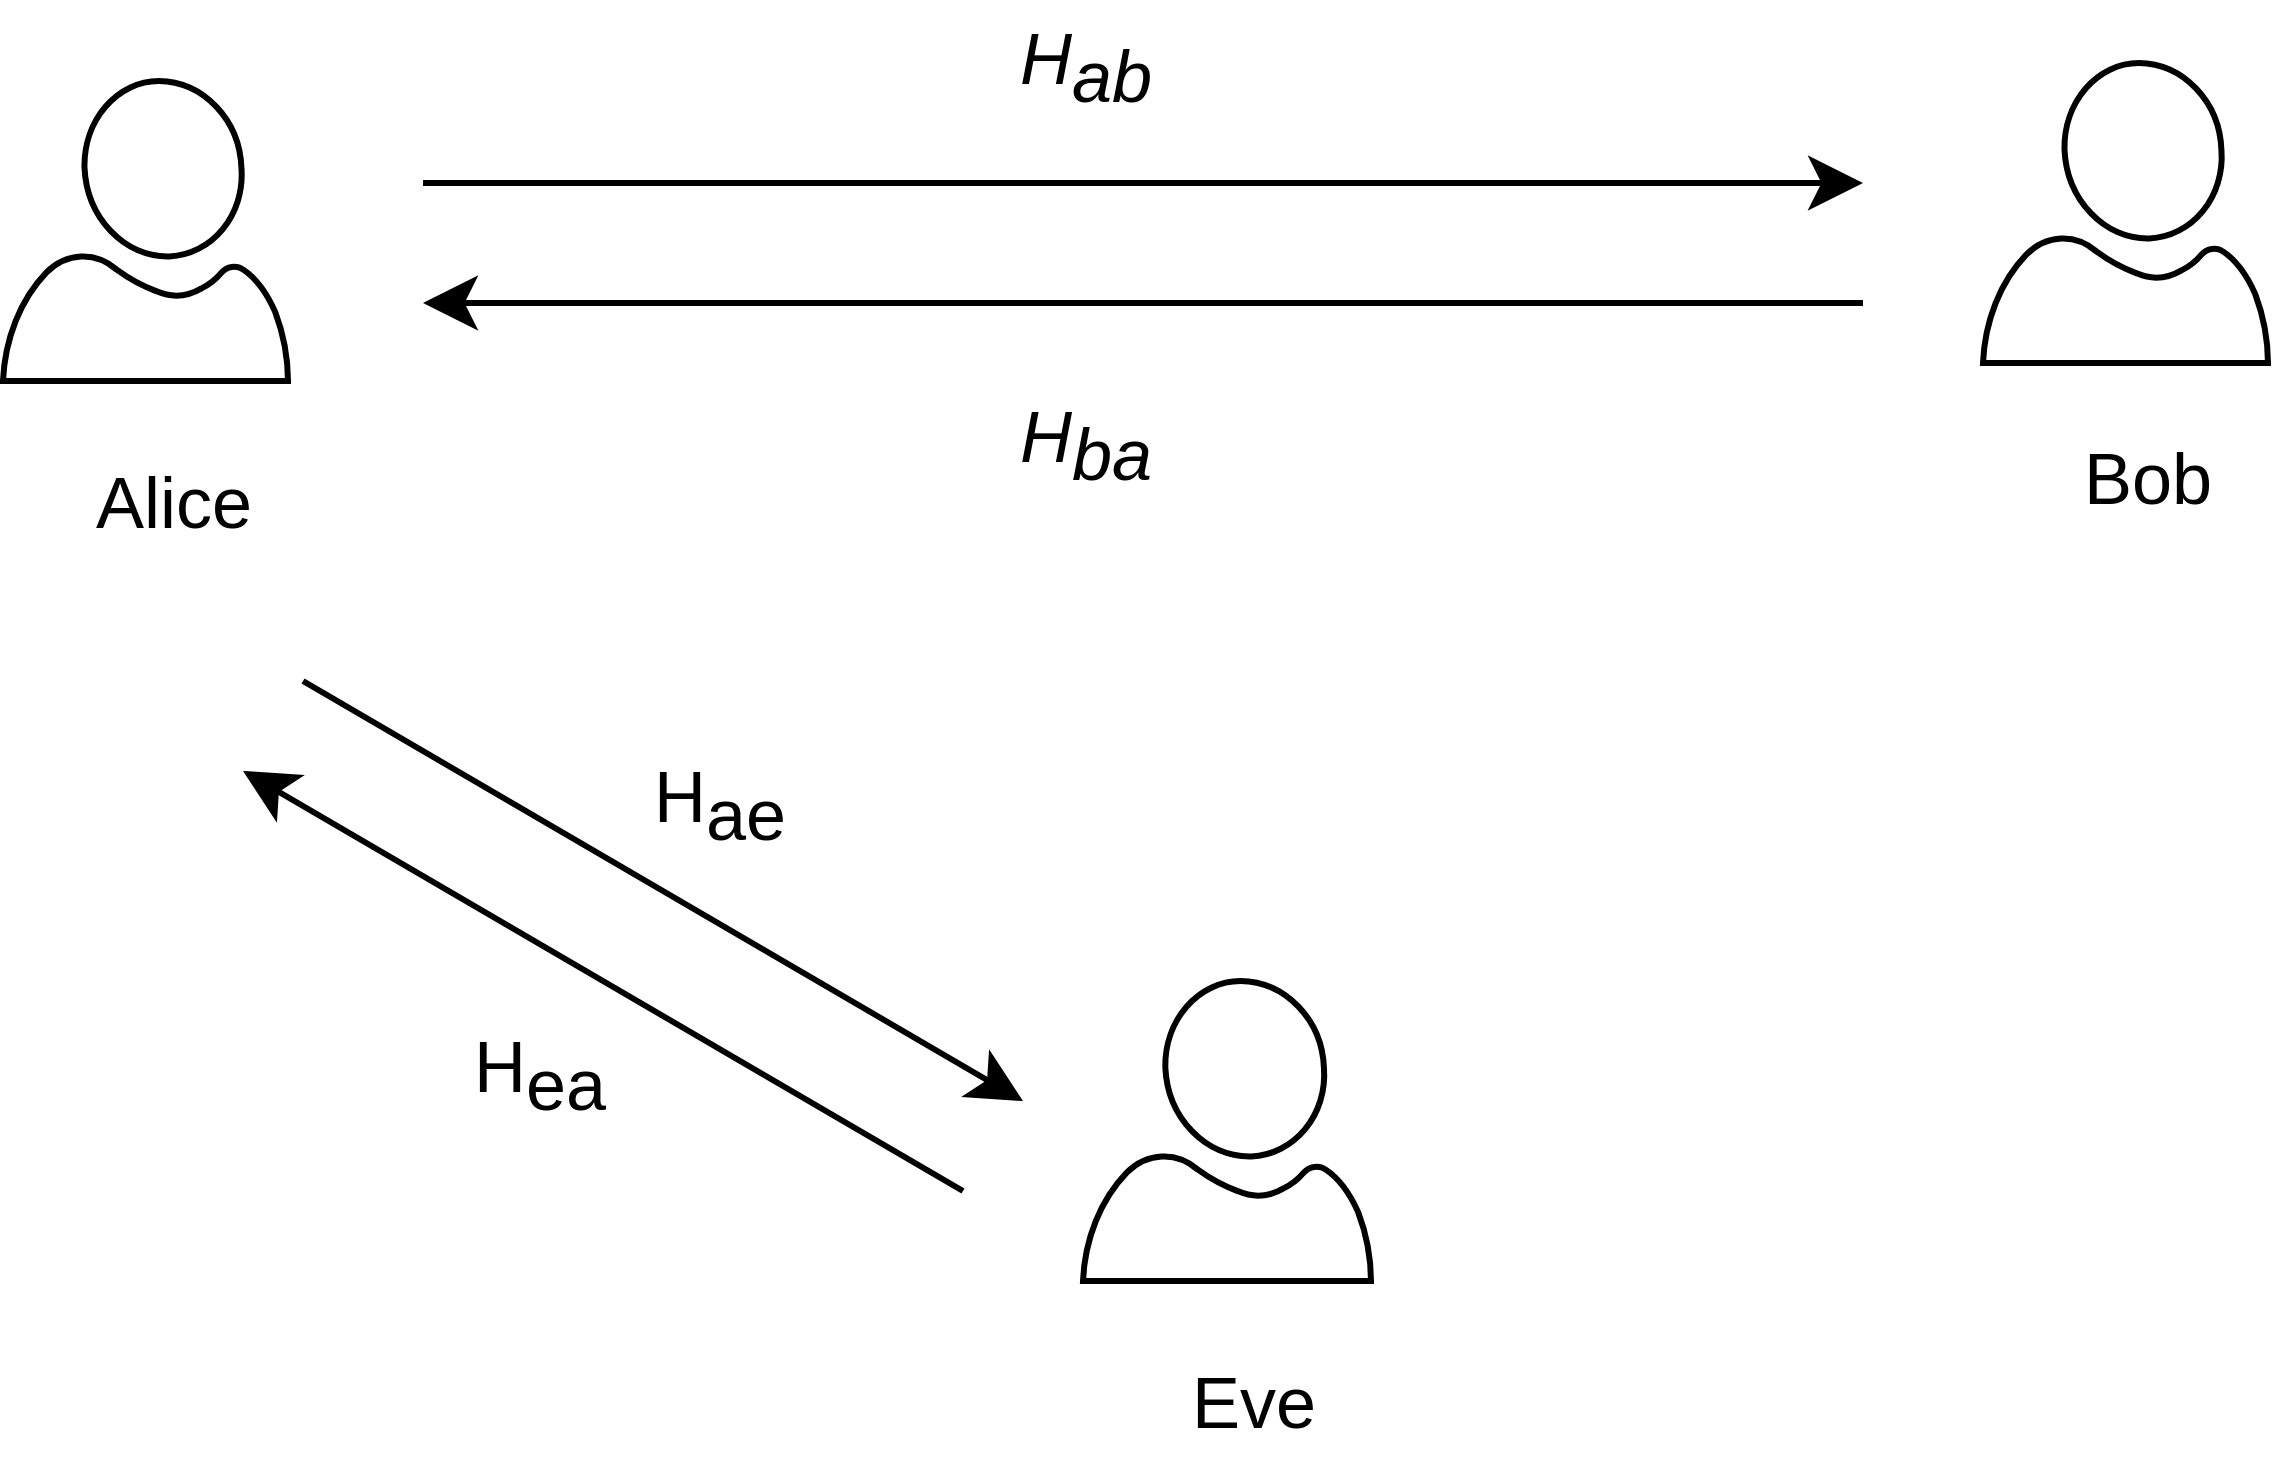
\includegraphics[width=0.9\textwidth]{images/channel} 
    \caption{无线通信信道}
    \label{wireless-channel}
\end{figure}

如图\ref{wireless-channel}所示,在某时刻t,通信双方Alice和Bob互相发射导频信号,在相干时间内,经管相同的多径信道衰落,对于窃听者Eve来说,无论是窃听来自Alice还是Bob的发射信号,其信道衰落都不同于Alice和Bob之间的信道衰落。在相干距离d(半波长)以外,Eve接收信号经历的多径衰落与Bob接收信号的多径衰落不再相关。除非攻击者在物理空间上靠近任意合法通信双方,否则无法分析出通信双方的CSI\cite{sasaoka2009secret}。

\subsection{无线信道的时变特性}

% 参考 3.1.1

信道衰落分为两类,大尺度衰落和小尺度衰落。大尺度衰落包括路径损耗和阴影损耗,在长距离传输(上百米)中,信号强度会发生变化。路径损耗指空间传播中电磁波的损耗,阴影损耗指在电磁波在传输过程中,受到遮挡物影响产生阴影效应,导致场强变化。通常用自由空间模型、Hata-Okumura,模型等来描述大尺度衰落。

小尺度衰落通常反应在短距离范围内信号幅值的变化中,通常符合瑞利分布、莱斯分布,小尺度衰落分为快衰落信道和慢衰落信道,快衰落信道又分为空间选择性快衰落信道、时间选择性快衰落信道、频率选择性快衰落信道。小尺度衰落反应无线信道的多径和时变,在无线通信中,通信双方之间信号经过的物理路径比较复杂,会收到多径的影响,可以将多径衰落信道建模成时变脉冲有限响应滤波器(FIR),即,

\begin{equation}
    h(\tau, t) = \sum_{l = 1}^{N(t)} a_k(t) \sigma(\tau - \tau_k(t))
\end{equation}

其中,t时刻,多径分量个数为$N(t)$,$a_k(t)$表示t时刻第l条路径信号幅度,$\tau_k(t)$表示t时刻第l条路径的延迟。

在一次信道探测过程中,若探测间隙大于信道的相干时间,接收信号经历快衰落过程,即时间选择性衰落。若信号带宽大于信道的相干带宽,接收信号经历频率选择性衰落,接收信号会产生符号间干扰(ISI)。


\section{密钥生成流程}

本文基于无线信道密钥生成技术设计的系统主要分为四个阶段,信道探测、特征量化、信息调和,整体架构如图\ref{whole_structure}所示。其中,Alice和Bob是合法通信双方,Eve是第三方窃听者。信道探测阶段是无线信道传输导频信号,信息调和阶段是通过公共信道传输调和信息。

\begin{figure}[htbp!]
    \centering 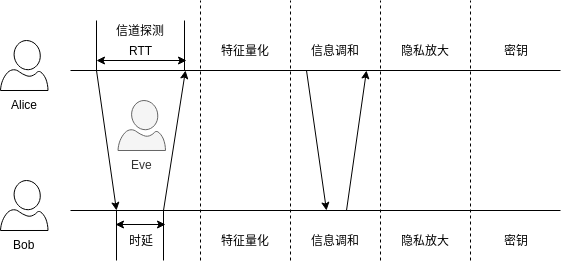
\includegraphics[width=0.9\textwidth]{images/whole_structure} 
    \caption{无线密钥生成流程的整体架构}
    \label{whole_structure}
\end{figure}

\subsection{信道探测}

在一个单入单出线性系统中,设脉冲响应函数为$g(k)$,根据维纳-霍夫方程的离散形式,发射信号$x(k))$和$y(k)$之间的相关函数为,

\begin{equation}
    R_{xy}(\tau)  = \sum_{j=0}^{\infty} g(j) R_x(\tau-j)\Delta t
\end{equation}

同时,M序列的自相关函数为,

\begin{equation}
    R_m(\tau) = \left\{
  \begin{aligned}
  &1, &\tau = 0, N, 2N, ... \\
  &-\frac{1}{N}, &wherelse \\
  \end{aligned}
  \right.
\end{equation}

因此,当发射信号x(k)为M序列时,即$x(k) = m(k)$时,有,

\begin{equation}
    R_{ym}(k) = \sum_{j=0}^{N-1} \tilde{g}(j)R_m(k-j)\Delta t
\end{equation}
\begin{equation}
    R_{ym}(k) = \frac{(N+1)\Delta t}{N} \tilde{g}(k) - \frac{\Delta t}{N} \sum_{j=0}^{N-1} \tilde{g}(j)
\end{equation}
  
\begin{equation}\label{eq1}
    \tilde{g}(k) = \frac{N}{(N+1)\Delta t} [R_{ym}(k) + c]
\end{equation}

其中,

\begin{equation}
  R_{ym}(k) = \frac{1}{N}\sum_{j=0}^{N-1}m(j-k)y(j)
\end{equation}

工程上,

\begin{equation}
  c=-R_{ym}(N_P - 1)
\end{equation}
  
在TDD/FDD系统中,用户Alice和Bob互相发送导频信号帧$m(t)$作为导频信号。设$h_{ab}$代表Alice到Bob信道的频率响应,$h_{ba}$代表Bob到Alice信道的频率响应。那么,

Alice检测的时域信号为,

\begin{equation}
    y_{ba}(t) = m(t) * h_{ba}(t) + n_{ba}(t) 
\end{equation}

Bob检测的时域信号为,

\begin{equation}
    y_{ab}(t) = m(t) * h_{ab}(t) + n_{ba}(t)    
\end{equation}

因此Bob通过式(\ref{eq1})估计信道,

\begin{equation}
    \tilde{h}_{ab}(k) = a\sum_{j=0}^{N-1}m(j-k)y_{ab}(j)
\end{equation}
  
同理,Alice通过式(\ref{eq1})估计信道,
  
\begin{equation}
    \tilde{h}_{ba}(k) = a\sum_{j=0}^{N-1}m(j-k)y_{ba}(j)
\end{equation}
  
其中,a为常数,

\begin{equation}
    a = \frac{2-N_p}{(N + 1)\Delta t}
\end{equation}

\subsection{预处理}

在步骤信道探测中,通信双方分别通过导频信号估计探测时隙$\tau$内的脉冲响应$\tilde{h}_{ba}$和$\tilde{h}_{ab}$,并进行快速傅里叶变换得到信道频率响应$\tilde{H}_{ba}$和$\tilde{H}_{ab}$。由于在探测过程中,无线信道测量结果会受到环境噪声、射频器件的非线性等因素影响,因此通常会进一步预处理来提高信道的互易性和消除数据冗余。

\begin{equation}
    \tilde{H}_{ba} = Pre(FFT(\tilde{h}_{ba}))
\end{equation}
\begin{equation}
    \tilde{H}_{ab} = Pre(FFT(\tilde{h}_{ab}))
\end{equation}

其中,$Pre$表示预处理函数,$FFT$表示快速傅里叶变换。

\subsection{特征量化}

目前有多种量化策略,常用的有单门限量化、多门限量化、自适应门限量化等。

文献\citet{aono2005wireless}采用如图\ref{single_quantization}所示的单门限量化,量化阈值取RSSI(Radio Signal Strength Indicator)平均值,可以带来比较高的密钥一致率,但是测量值在阈值附近时容易量化错误,并且由于量化精度不高,在信道变化缓慢时,生成密钥容易出现大量连续0比特和1比特长串。

\begin{figure}[htbp!]
    \centering 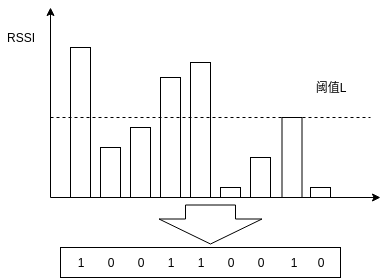
\includegraphics[width=0.9\textwidth]{images/single_quantization} 
    \caption{单门限量化}
    \label{single_quantization}
\end{figure}

文献\citet{mathur2008radio}采用如图\ref{two_quantization}所示双门限量化,将门限$L^+$和$L^-$之间的值舍弃,将$L^+$以上的值量化为1,将$L^-$以下的值量化为0,通信双方会在公共信道上交互传输未舍弃比特位的索引信息,因此第三方窃听者只有可能得知哪些比特被使用而无法得知被量化成0还是1,但是会降低密钥生成速率。

\begin{figure}[htbp!]
    \centering 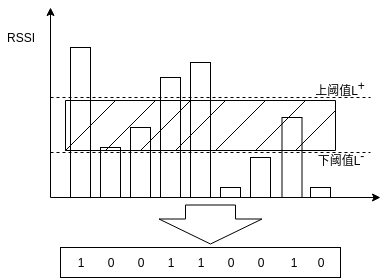
\includegraphics[width=0.9\textwidth]{images/two_quantization} 
    \caption{双门限量化}
    \label{two_quantization}
\end{figure}

文献\citet{patwari2009high}通过多次测量表明双门限量化每次会丢失5\%至27\%的比特数,并提出多比特自适应量化方法。文献\citet{yasukawa2008secret}使用多级量化,先将RSSI根据大小排序,然后分割成等间隔的$N = 2^m$块,m是量化比特数,并且通常$N \leq log_2^{maxValue}$,这样每个量化阶值的出现率是相同的。

通常多比特量化之后,会进一步编码成对应阶数格雷码。格雷码的特性是,相邻位置的格雷码只有一个位置的比特不同,因此使用格雷码可以提高通信双方的密钥一致率。无论是上述哪种量化方法,都避免不了密钥生成率和密钥一致性之间的矛盾。量化阶数越高,量化比特数越多,密钥生成率越高,但误差影响较大,密钥一致率降低;量化阶数越低,量化比特数越少,密钥一致率越高,但是密钥生成速率越低。

本文使用均匀量化的方法。在一次密钥生成过程中,Alice和Bob分别探测信道、预处理得到CSI。先对CSI降采样,以降低密钥泄漏率\cite{linning2019investigation}。同时,量化可以降低噪声的影响\cite{wang2015survey}。设量化时CSI最大值为$m_{max}$,量化阶数为R,量化前的值为m,量化后的值为q,将CSI归一化后按照式\ref{quantization_formula}均匀量化,得到离散的采样值,采样值对应比特数即量化阶数,本文量化阶数为3。密钥的生成速率与量化阶数成正比,通信双方的密钥一致率与量化阶数成反比。因此可以根据信噪比去调整量化阶数以得到较为均衡的密钥生成速率与一致率。量化之后的采样值需要进一步格雷编码降低密钥的不一致率。然后进行8b10b编码,过程如图\ref{quantization}所示。

\begin{equation} \label{quantization_formula}
    q = \frac{m_{max} * m}{2^{max}}
\end{equation}

\section{无线信道密钥的评估标准}

\chapter{TDD系统信道探测系统研究设计}
\chapter{FDD系统信道探测系统研究设计}
\chapter{无线信道密钥生成流程}

\chapter{实验和数据}
\section{描述性分析}
\section{实证分析}
\section{实证小结}

\chapter{总结展望}

\end{Main} % 结束正文

\begin{Acknowledgement}{}
这次的毕业论文设计总结是在我的指导老师xxx老师亲切关怀和悉心指导下完成的。从毕业设计选题到设计完成,x老师给予了我耐心指导与细心关怀,有了莫老师耐心指导与细心关怀我才不会在设计的过程中迷失方向,失去前进动力。x老师有严肃的科学态度,严谨的治学精神和精益求精的工作作风,这些都是我所需要学习的,感谢x老师给予了我这样一个学习机会,谢谢!

  感谢与我并肩作战的舍友与同学们,感谢关心我支持我的朋友们,感谢学校领导、老师们,感谢你们给予我的帮助与关怀;感谢肇庆学院,特别感谢计算机科学与软件学院四年来为我提供的良好学习环境,谢谢!
\end{Acknowledgement}

% 参考文献
\bibliography{seuthesis}



\newpage
\printindex % 索引

%\begin{thebibliography}{99}


% \bibliographystyle{ieee}
% \bibliography{seuthesis}


\end{document}
